\chapter{Fundamentação Teórica} \label{cap:fund}

%Falta escrever essa parte.
\section{Inteligência Artificial} \label{cap:fund-ia}

Apesar de ter chamado atenção nos últimos anos com a quantidade enorme de dados adquiridos e processados por grandes corporações como Google, Facebook, Amazon, e Apple \cite{ref:Lawless-Mittu-Sofge}, o termo `Inteligência Artificial' não é tão atual assim. Ele foi utilizado pela primeira vez em 1955 por John McCarthy \cite{ref:Cohen}, que conduziu no ano seguinte um workshop cuja premissa central da proposta considera que o comportamento humano inteligente consiste em processos que podem ser formalizados e reproduzidos por uma máquina \cite{ref:Harvard-AI}. %conjectura

Um dos objetivos da Inteligência Artificial, de acordo com \citeonline{ref:Mitchell-Michalski-Carbonell}, é fazer com que computadores realizem tarefas mais inteligentes de forma com que não haja necessidade dos seres humanos executá-las. Entretanto, um dos grandes desafios da área de IA atualmente é a execução de atividades consideradas simples e corriqueiras para pessoas, como reconhecimento de objetos e fala \cite{ref:Goodfellow-Bengio-Courville}. Para ilustrar isso, a tabela da \autoref{fig:fund-dificuldades} apresenta a diferença entre o nível de dificuldade que um computador ou ser humano tem para resolver determinado problema.

\begin{figure}[h!] %H
  \centering
  \caption{Exemplos de problemas e seus níveis de complexidade para computadores ou seres humanos resolvê-los.}
  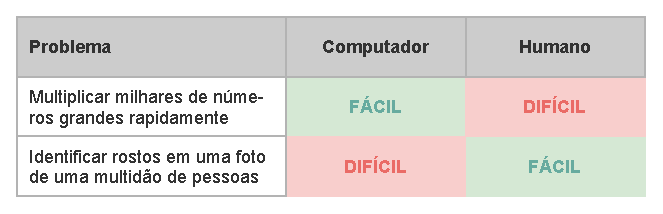
\includegraphics[scale=1.1]{img/img-fundamentacao-dificuldades.pdf}
  \label{fig:fund-dificuldades}
  \indentedfont[15.2cm]{Adaptado de \citeonline{ref:Rashid}}
\end{figure}

A Inteligência Artificial engloba a área de estudo do Aprendizado de Máquina, que por sua vez englobam as áreas do Aprendizado de Representação e Aprendizado Profundo, conforme o diagrama de Venn apresentado na \autoref{fig:fund-ia}.

\begin{figure}[h!] %H
  \centering
  \caption{Diagrama de Venn da Inteligência Artificial e suas áreas de estudo. }
  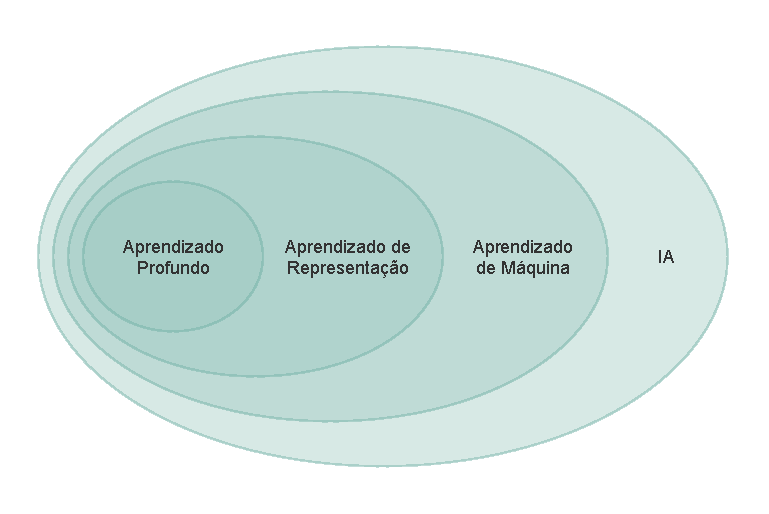
\includegraphics[scale=1.1]{img/img-fundamentacao-ia.pdf}
  \label{fig:fund-ia}
  \indentedfont[15.2cm]{Adaptado de \citeonline{ref:Goodfellow-Bengio-Courville}}
\end{figure}

Para evidenciar as diferenças entre essas áreas de estudo, em comparação com simples Sistemas Baseados em Regras, \citeonline{ref:Goodfellow-Bengio-Courville} apresenta um fluxograma com as etapas de processamento entre a entrada e a saída de dados para cada uma delas, presente na \autoref{fig:fund-fluxograma}.

\begin{figure}[h!] %H
  \centering
  \caption{Fluxograma que diferencia as áreas de estudo da Inteligência Artificial e suas etapas de processamento de dados. }
  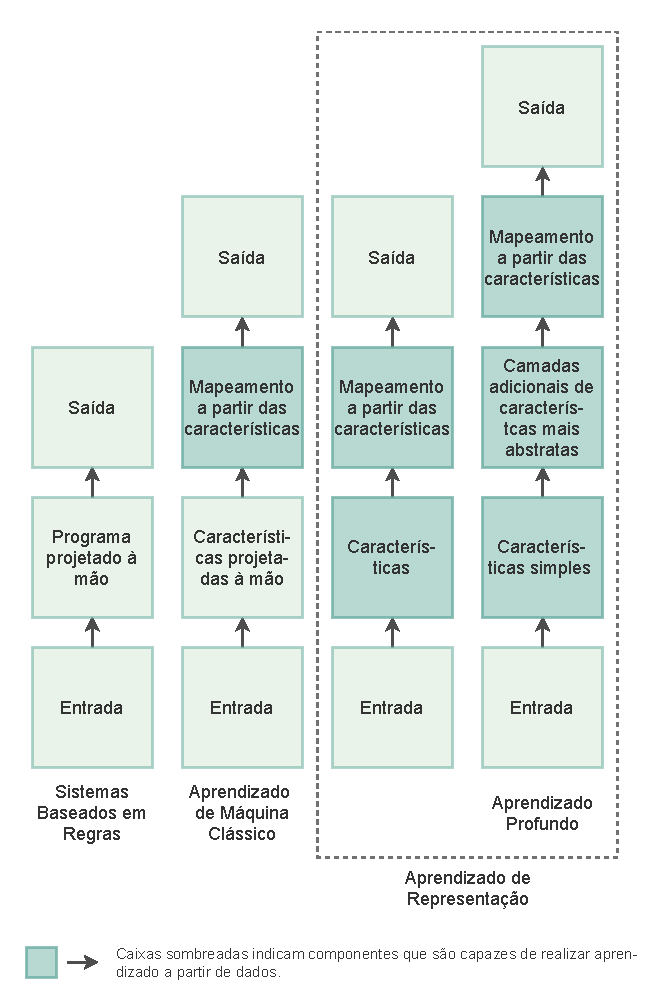
\includegraphics[scale=1.1]{img/img-fundamentacao-fluxograma.pdf}
  \label{fig:fund-fluxograma}
  \indentedfont[15.2cm]{Adaptado de \citeonline{ref:Goodfellow-Bengio-Courville}}
\end{figure}

Sistemas Baseados em Regras não possuem componentes capazes de realizar qualquer aprendizado a partir e dados \cite{ref:Goodfellow-Bengio-Courville} e são utilizados para resolução de problemas e/ou execução de tarefas que podem ser descritos por uma lista de regras formais, como por exemplo jogar Xadrez. Ao contrários desses sistemas, o Aprendizado de Máquina (do inglês \textit{Machine Learning}) utiliza algoritmos computacionais para transformar características reunidas empiricamente em modelos utilizáveis \cite{ref:Edgar-Manz} possuindo a capacidade ``de se aprimorar [...], aprendendo novos conhecimentos ao invés de serem programado com eles'' \cite{ref:Woolf}.

No Aprendizado de Representação (do inglês \textit{Feature Learning} ou \textit{Representation Learning}) entretanto, não há necessidade de mapear manualmente essas características \cite{ref:Goodfellow-Bengio-Courville}. Ou seja, por conta própria e de forma abstrata, os algoritmos são capazes de extrair as características importantes para a construção dos modelos utilizando redes neurais \cite{ref:Robins} \cite{ref:Lesort}. O Aprendizado Profundo, por sua vez, resolve a dificuldade que o Aprendizado de Representação possui de extrair características abstratas de alto nível, tais como sotaques de um locutor \cite{ref:Goodfellow-Bengio-Courville}. Segundo \citeonline{ref:Mao-Wang-Tang-Qian}, o Aprendizado Profundo ``imita a função que o cérebro humano possui de interpretar dados usando redes neurais de várias camadas''. Um exemplo dessas variadas camadas é apresentado na \autoref{fig:fund-camadas}, onde características distintas são extraídas por cada camada. Uma comparação com o modelo de Aprendizado de Máquina é ilustrado na \autoref{fig:fund-aprendizados}.

\begin{figure}[h!] %H
  \centering
  \caption{Ilustração das camadas de um modelo de Aprendizado Profundo.}
  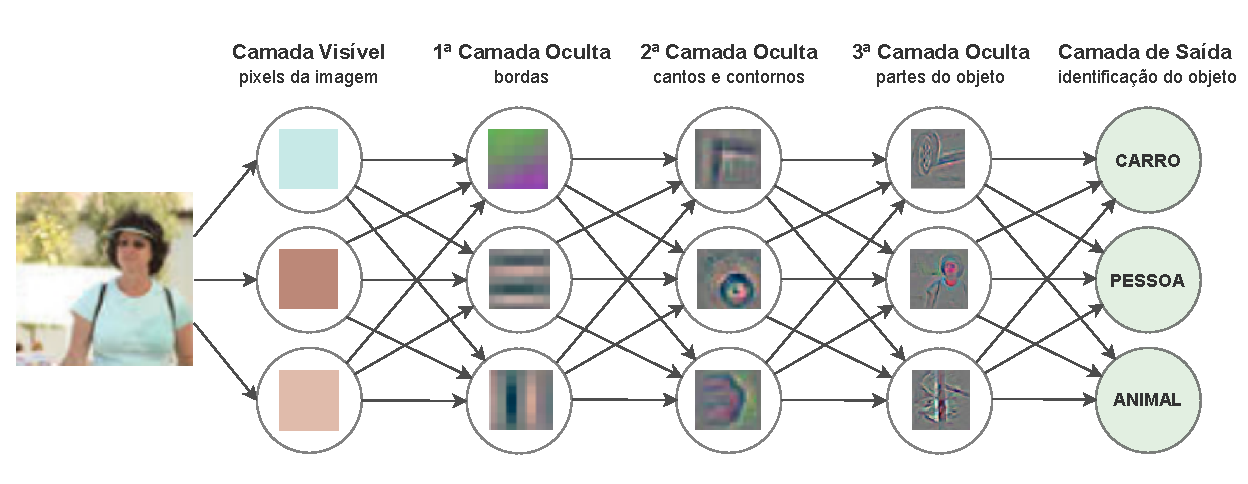
\includegraphics[scale=0.8]{img/img-fundamentacao-deep-learning.pdf}
  \label{fig:fund-camadas}
  \indentedfont[15.2cm]{Adaptado de \citeonline{ref:Goodfellow-Bengio-Courville}}
\end{figure}

\begin{figure}[h!] %H
  \centering
  \caption{Comparação entre os modelos Aprendizado de Máquina e Aprendizado Profundo.}
  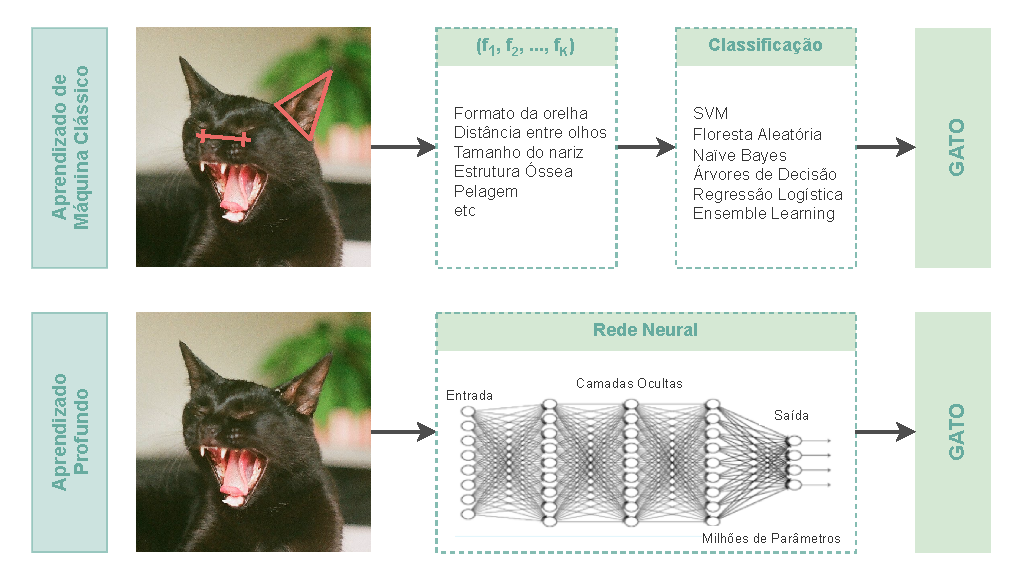
\includegraphics[scale=0.95]{img/img-fundamentacao-aprendizados.pdf}
  \label{fig:fund-aprendizados}
  \indentedfont[15.2cm]{Adaptado de \citeonline{ref:Robins}}
\end{figure}

\section{Redes Neurais} \label{cap:fund-ia-rn}
Ao contrário da abordagem convencional de programação, onde dizemos a um computador o que deve ser feito ao dividir um problema em pequenas tarefas para que ele execute, uma Rede Neural (do inglês \textit{Neural Network}) utiliza dados observacionais para aprender como resolver o problema \cite{ref:Nielsen}.

\citeonline{ref:Walczak-Cerpa} define Redes Neurais Artificiais como modelos que ``simulam a atividade elétrica do cérebro e do sistema nervoso''. Porém enquanto alguns tipos de redes neurais tem sido utilizadas para entender o funcionamento do cérebro, na perspectiva de Aprendizado Profundo elas não são projetadas para serem modelos realistas da função biológica \cite{ref:Goodfellow-Bengio-Courville}.

\subsection{Estrutura de Uma Rede Neural} \label{cap:fund-ia-rn-estrutura}
Uma Rede Neural é composta por camadas de nós, conhecidos como neurônios, e conexões que interligam as saídas e entradas desses nós. A estrutura básica de uma Rede Neural é ilustrada na \autoref{fig:fund-nn}, onde a primeira camada de neurônios é a camada de entrada, a última camada é a camada de saída e as camadas entre elas são chamadas de camadas ocultas. Na \autoref{fig:fund-nn}, vetor $\mathrm{X}$ contém os valores de entrada, os vetores $\mathrm{a^{[l]}}$ representam as funções de ativação referentes à \textit{l-ésima} camada, e $\mathrm{\hat{y}}$ é o vetor de saída com os valores preditos. As notações utilizadas nesse capítulo respeitam as propostas por \citeonline{ref:Ng} presentes no \autoref{apendice:notacao}.

\begin{figure}[h!] %H
  \centering
  \caption{Estrutura básica de uma Rede Neural com duas camadas.}
  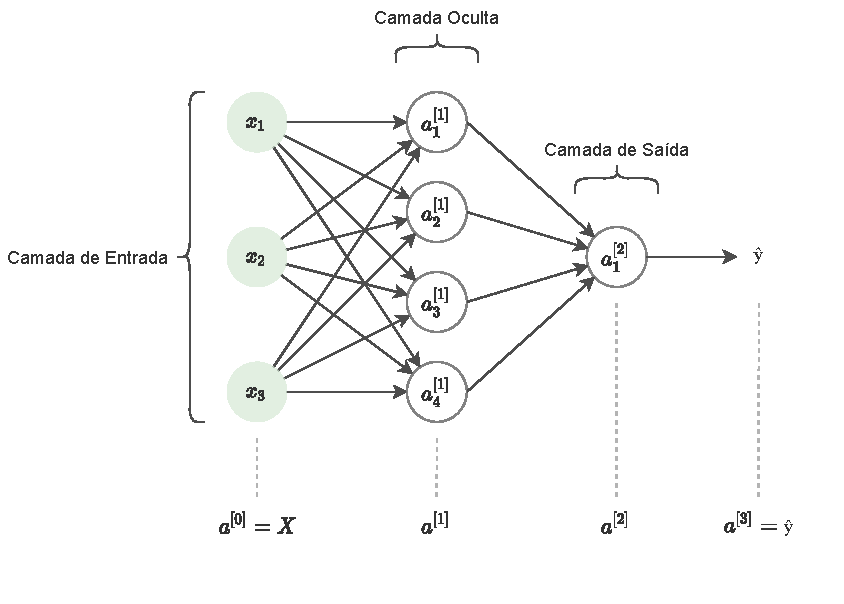
\includegraphics[scale=1.1]{img/img-fundamentacao-nn.pdf}
  \label{fig:fund-nn}
  \indentedfont[15.2cm]{Elaboração própria (2021)}
\end{figure}

São nos neurônios que ocorrem as computações. A \autoref{fig:fund-no} mostra um diagrama de um nó de uma Rede Neural, onde os pesos representados por b e $\mathrm{w_k}$ são responsáveis por atribuir significância às entradas com relação à tarefa que o algoritmo está tentando aprender \cite{ref:Nicholson}. Esses produtos são então somados e passam por uma função de ativação.

\begin{figure}[h!] %H
  \centering
  \caption{Diagrama de um Neurônio de uma Rede Neural.}
  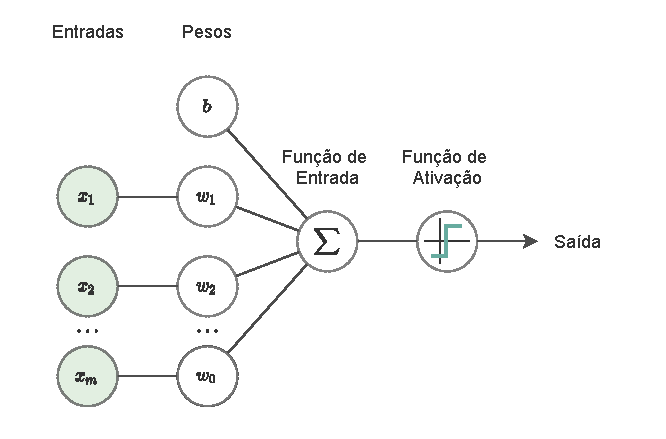
\includegraphics[scale=1.1]{img/img-fundamentacao-no.pdf}
  \label{fig:fund-no}
  \indentedfont[15.2cm]{Adaptado de \citeonline{ref:Nicholson}}
\end{figure}

\subsection{Funções de Ativação} \label{cap:fund-ia-rn-func}
As funções de ativação desempenham um papel crucial na dinâmica de desempenho e treinamento em redes neurais \cite{ref:Misra}, determinando se um sinal deve progredir e em que medida ele deve progredir através da rede \cite{ref:Nicholson}. Alguns exemplos de função de ativação estão na \autoref{fig:fund-funcs}.

\begin{figure}[h!]
    \centering
    \caption{Exemplos de funções de ativação de um neurônio para uma Rede Neural.}
    \begin{subfigure}[H]{.4\textwidth}
        \centering
        \caption{Sigmóide}
        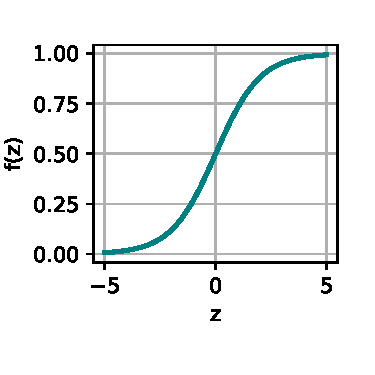
\includegraphics[scale=0.8]{img/img-fundamentacao-sig.pdf}
        \label{fig:fund-funcs-sig}
    \end{subfigure}
    \begin{subfigure}[H]{.4\textwidth}
        \centering
        \caption{Tangente Hiperbólica}
        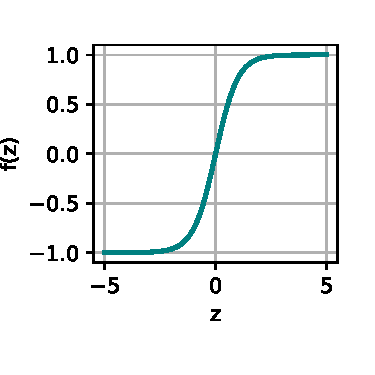
\includegraphics[scale=0.8]{img/img-fundamentacao-tanh.pdf}
        \label{fig:fund-funcs-tanh}
    \end{subfigure}
    \begin{subfigure}[H]{.4\textwidth}
        \centering
        \caption{ReLU}
        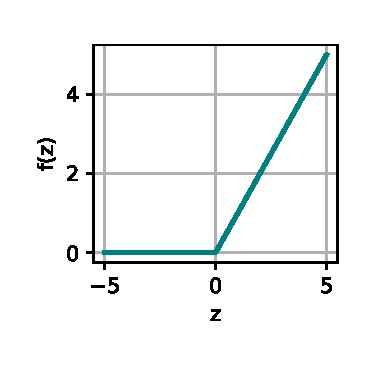
\includegraphics[scale=0.8]{img/img-fundamentacao-relu.pdf}
        %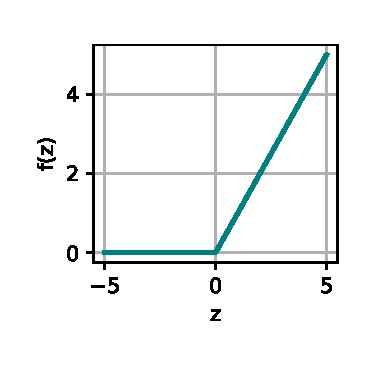
\includegraphics[width=\textwidth]{img/img-fundamentacao-relu.pdf}
        \label{fig:fund-funcs-relu}
    \end{subfigure}
    \begin{subfigure}[H]{.4\textwidth}
        \centering
        \caption{Mish}
        %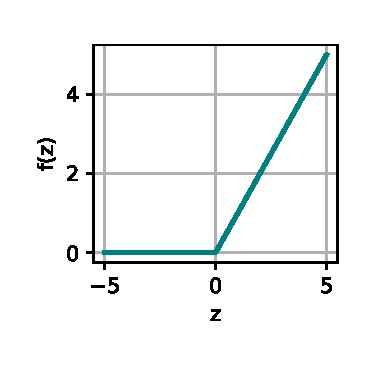
\includegraphics[scale=0.8]{img/img-fundamentacao-relu.pdf}
        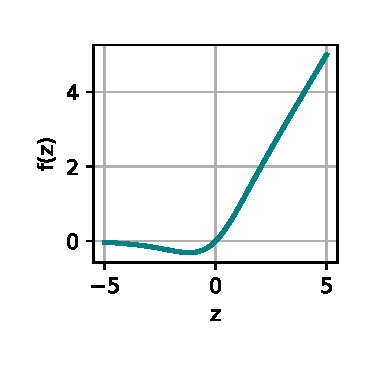
\includegraphics[scale=0.8]{img/img-fundamentacao-mish.pdf}
        \label{fig:fund-funcs-mish}
    \end{subfigure}
    \indentedfont[15.5cm]{Elaboração própria (2021)}
	\label{fig:fund-funcs}
\end{figure}

A função Sigmóide da \autoref{fig:fund-funcs-sig}, definida por \citeonline{ref:Sharma} pela \autoref{eq:fund-sig}, é geralmente utilizada em classificações binárias, pois o resultado está sempre no intervalo entre zero e um \cite{ref:Ng}.

\begin{equation} \label{eq:fund-sig}
  \text{f(z)} = \sigma(z) = \frac{1}{1 + e^{-z}}
\end{equation}

Para a otimização dos pesos durante o treinamento de uma rede neural, em geral é necessário calcular o gradiente das funções de ativação. Por isso, de acordo com \citeonline{ref:Sharma}, o uso da tangente hiporbólica como função de ativação é preferível pois tem gradientes que não estão restritos a variar em uma certa direção e são mais acentuados quando comparado à Sigmóide. A definição da tangente hiporbólica da \autoref{fig:fund-funcs-tanh} está na \autoref{eq:fund-tanh}.

\begin{equation} \label{eq:fund-tanh}
  \text{f(z)} = tanh(z) = \frac{e^{z} - e^{-z}}{e^{z} + e^{-z}}
\end{equation}

Porém, para valores muito grandes ou muito pequenos de $\mathrm{z}$, a derivada resultante, utilizada no gradiente, tende a ser nula tanto para a sigmóide quanto para a tangente hiperbólica \cite{ref:Ng} o que geralmente causa lentidão no treinamento \cite{ref:Misra}. Para que isso não ocorra, utiliza-se a função ReLU, do inglês \textit{Rectified Linear Unit}, plotada na \autoref{fig:fund-funcs-relu} e definida na \autoref{eq:fund-relu}. A ReLU é a função de ativação mais utilizada \cite{ref:Ng} e é a função padrão recomendada para uso com a maioria das redes neurais \cite{ref:Goodfellow-Bengio-Courville}.

\begin{equation} \label{eq:fund-relu}
  \mathrm{{f(z)} = ReLU(z) = max(0, z)}
\end{equation}

Com a evolução das Redes Neurais na última década, diversas funções de ativação vem sendo propostas com o objetivo de melhorar o desempenho do treinamento. Um exemplo delas é a Mish (\autoref{fig:fund-funcs-mish}), proposta por \citeonline{ref:Misra} cuja função é definida pela \autoref{eq:fund-mish}.

\begin{equation} \label{eq:fund-mish}
  \mathrm{{f(z)} = z \cdot tanh(ln(1 + e^z))}
\end{equation}

Segundo \citeonline{ref:Misra}, ao contrário da ReLU, a função Mish é continuamente diferenciável, evitando efeitos colaterais indesejados quando utiliza-se a otimização baseada no método do gradiente.

\subsection{Treinamento de Uma Rede Neural}\label{cap:fund-ia-rn-treinamento}

Para o treinamento de uma Rede Neural, utiliza-se um conjunto de exemplos de treinamento $\{(x^{(1)}, y^{(1)}), \cdots, (x^{(m)}, y^{(m)})\}$, onde $x^{(i)}, y^{(i)}$ são, respectivamente, a entrada e a saída real do \textit{i-ésimo} exemplo de treinamento de um conjunto contendo m exemplos de treinamento \cite{ref:Ng}. Para cada um desses exemplos, o objetivo é fazer o cálculo dos pesos w e b de forma que a saída estimada $\hat{y}^{(i)}$ seja próxima da saída real $y^{(i)}$.

O peso b é chamado de \textit{bias} e não é multiplicado a nenhum valor da entrada para caso todos os valores de x sejam nulos, a saída $\hat{y}^{(i)}$ seja diferente de zero. O cálculo desses pesos é feito de forma iterativa e geralmente são iniciados de forma aleatória.

O processo de cálculo considerando um nó de uma rede neural está ilustrado na \autoref{fig:fund-etapas}, onde a função de ativação utilizada é a sigmoide e todos os valores calculados e os de entrada são representados na forma vetorial.

\begin{figure}[h!] %H
  \centering
  \caption{Estapas da atualização dos pesos de um nó em uma Rede Neural.}
  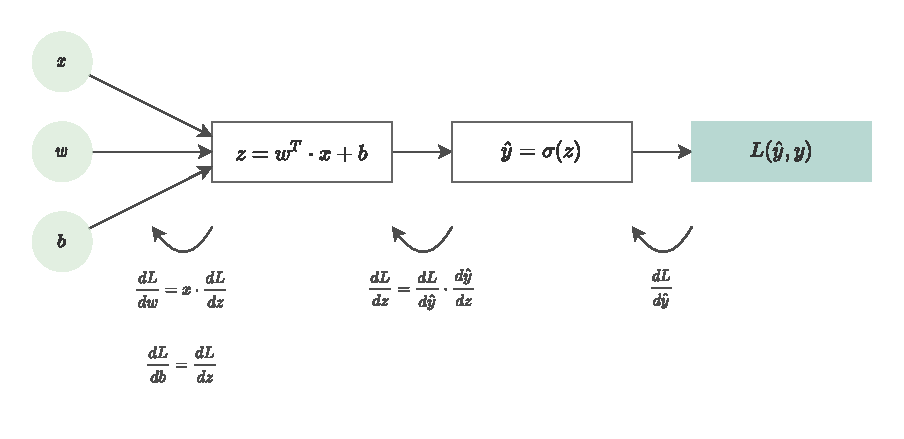
\includegraphics[scale=1.1]{img/img-fundamentacao-etapas.pdf}
  \label{fig:fund-etapas}
  \indentedfont[15.2cm]{Adaptado de \citeonline{ref:Ng}}
\end{figure}

A primeira etapa a ser computada após a passagem das entradas pela função de ativação é função de perda, que mede quão boa é a saída prevista $\hat{y}$ em comparação aos valores verdadeiros de y para apenas um conjunto de treinamento \cite{ref:Ng}.

Um exemplo de função de perda que compara $\mathrm{\hat{y}}$ com y pode ser definida pela \autoref{eq:fund-perda} \cite{ref:Ng}, onde o objetivo do treinamento é obter $L(y,\hat{y}) = 0$.

\begin{equation} \label{eq:fund-perda}
  \mathrm{
    L(y,\hat{y}) = -(y \cdot log(\hat{y}) + (1 - y) \cdot log(1 - \hat{y}))
  }
\end{equation}

Dessa forma, como $\mathrm{\hat{y} = f(w, b)}$, é necessário encontrar valores para os pesos w e b que minimizem a função de perda $L(y,\hat{y})$. Para isso, utiliza-se o método do gradiente, um algoritmo de primeira ordem iterativo utilizado em otimização para encontrar o mínimo local de uma função \cite{ref:Yan}, exemplificado na \autoref{fig:fund-gradiente} para uma função de perda considerando apenas a variável w.

\begin{figure}[h!] %H
  \centering
  \caption{Método do gradiente para uma variável.}
  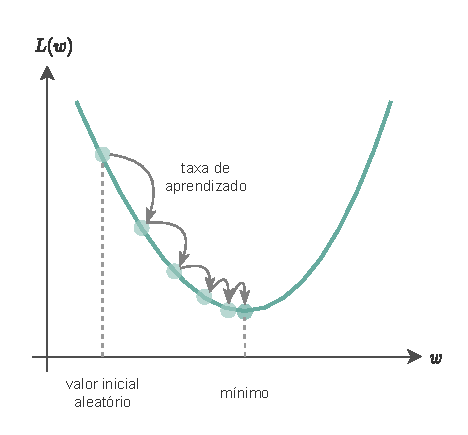
\includegraphics[scale=1.3]{img/img-fundamentacao-gradiente.pdf}
  \label{fig:fund-gradiente}
  \indentedfont[15.2cm]{Adaptado de \citeonline{ref:Sauer}}
\end{figure}


Após serem computadas as derivadas da \autoref{fig:fund-etapas}, os pesos w e b são atualizados conforme a \autoref{eq:fund-atualizacao-w} e a \autoref{eq:fund-atualizacao-b} onde $\alpha$ representa uma taxa de aprendizado \cite{ref:Ng}.

\begin{equation} \label{eq:fund-atualizacao-w}
  \mathrm{
    w = w - \alpha \cdot \frac{dL}{dw}
  }
\end{equation}

\begin{equation} \label{eq:fund-atualizacao-b}
  \mathrm{
    b = b - \alpha \cdot \frac{dL}{db}
  }
\end{equation}

A atualização desses pesos é feita até que a função de perda resulte valores muito próximos de zero.

\subsection{Redes Neurais Convolucionais} \label{cap:fund-ia-rn-prof}
Redes Neurais Profundas são caracterizadas por sua grande quantidade de camadas ocultas. Cada uma das camadas é responsável pelo treinamento de um conjunto distinto de dados com base na saída da camada anterior, de forma que quanto mais há avanço pela rede neural, mais complexos são as características que os nós podem reconhecer \cite{ref:Nicholson}, como ilustra a \autoref{fig:fund-camadas}.

Redes Neurais Convolucionais são um tipo de rede neural profunda originalmente projetadas para análise de imagens \cite{ref:Eden-Ierapetritou-Towler}.
%CNN is a deep neural network originally designed for image analysis
\subsubsection{\textit{You Only Look Once}} \label{cap:fund-ia-rn-conv}
\section{Classificação e Detecção de defeitos} \label{cap:fund-frameworks}
\section{Frameworks e Bibliotecas} \label{cap:fund-frameworks}
\subsection{OpenCV} \label{cap:fund-frameworks-opencv}
\subsection{Darknet} \label{cap:fund-frameworks-darknet}
\subsection{Flask} \label{cap:fund-frameworks-flask}
